% command to make sure colorboxes don't create whitespace between code lines

% Farben für jede Schicht
\newcommand{\applicationLayerColor}{Gold}
\newcommand{\transportLayerColor}{ForestGreen}
\newcommand{\networkLayerColor}{RoyalBlue}
\newcommand{\dataLinkLayerColor}{Gray}

\fboxsep=.6pt

% default settings for listings
\lstset{style=python}

\title[Internet]{Internet}

%\subtitle{Schichtenmodell und Protokolle}

\author[Wendl, Cyril] % (optional)
{Cyril Wendl}

\institute[KLW] % (optional)
{
    Fachschaft Informatik\\
    Kantonsschule im Lee
}

\date[\today] % (optional)

\logo{
\includegraphics[width=2cm]{Logos/LeeLogo}}

\titlegraphic{\vspace{-.7cm}\includegraphics[width=\textwidth]{"Grundlagen_Info/06_Datenbanken/Figures/title-emojis"}}

\frame{\titlepage}

\newcommand{\fldNum}{\refstepcounter{FormCounter}\raisebox{-0.28\normalbaselineskip}{\TextField[name=\theFormCounter, width=2cm,print,borderwidth=0, backgroundcolor={0.9 0.9 0.9}]{}}}

\begin{frame}{Netzwerk-Spiel (ca. 5')}
    Sie sind ein Computer im Internet und möchten gerne eine Nachricht an einen anderen Computer senden:
    \begin{center}
        \begin{tcolorbox}[colframe=\networkLayerColor, colback=white, boxrule=1pt, arc=4pt, left=2pt, right=2pt, top=2pt, bottom=2pt]
            \begin{table}[H]
                \tiny
                \centering
                \begin{tabular}{l|l}
                    \coin{3} Von:       & \texttt{192.168.0.\fldNum}                                                           \\\midrule
                    \coin{3} An:        & \texttt{192.168.0.\fldNum}                                                           \\\midrule
                    \coin{2} Sequenz:   & \texttt{\TextField[width=5cm, print,borderwidth=0, backgroundcolor={0.9 0.9 0.9}]{}} \\\midrule
                    \coin{1} Nachricht: & \TextField[width=5cm,print,borderwidth=0, backgroundcolor={0.9 0.9 0.9}]{}           \\
                \end{tabular}
            \end{table}
        \end{tcolorbox}
    \end{center}
    \textbf{Anleitung}\small
    \begin{itemize}[<+->]
        \item (Bereits gemacht): Notieren Sie sich eine einzigartige IP-Adresse für Ihren Computer, startend mit \texttt{192.168.0.xyz} (z.B. \texttt{192.168.0.3}), wobei  $\texttt{xyz} \in [0,255]$
        \item[\coin{1}] (Vorderseite) Schreiben Sie eine Nachricht (max. 10 Zeichen pro Karte)
        \item[\coin{2}] (Vorderseite) Nummerieren Sie die Karten in der Reihenfolge, in der sie gesendet werden sollen (Sequenz)
        \item[\coin{3}] (Rückseite) Fügen Sie die IP-Adressen der Absender- und Empfänger-Computer hinzu.
        \item[\faTruck] Übergeben Sie die Karten dem \enquote{Router} (= \enquote{Postbote})
    \end{itemize}
\end{frame}

\begin{frame}[fragile]{Was sind Netzwerke?}
    \begin{itemize}[<+->]
        \item Graphen:
              \begin{figure}[H]
                  \centering
                  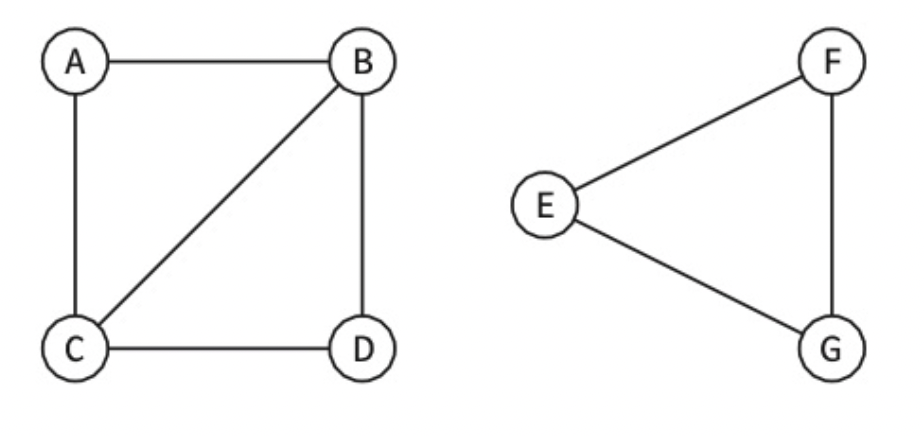
\includegraphics[keepaspectratio, width=0.35 \paperwidth]{Grundlagen_Info/02_Graphen/Figures/4-graph-zusammenhaengend.png}
              \end{figure}

        \item Im Alltag:
              \begin{itemize}
                  \item Kommunikations-Netzwerke: Die Post, DHL, Planzer, ...
                  \item Soziale Netzwerke: TikTok, Youtube, Instagram, ...
                  \item Transport-Netzwerke: SBB, Flixbus, ...
                  \item Shopping-Netzwerke: Aliexpress, Uber, ...
                  \item Computer-Netzwerke: \textbf{Das Internet}
              \end{itemize}
    \end{itemize}
\end{frame}

\begin{frame}[fragile]{Schichtenmodell}{Analogie}
    \begin{figure}[H]
        \centering
        \begin{tikzpicture}[
                auto,
                block/.style={
                        minimum width=3cm,
                        node distance=1.5cm,
                        rectangle,
                        fill=\networkLayerColor!50,
                        align=center,
                        rounded corners
                    }
            ]


            % Define the nodes with FontAwesome icons
            \node[block] (chefs) {\faFemale\ Chef};
            \node[block, below=of chefs] (secretariat) {\faPhone\ Sekretariat};
            \node[block, below=of secretariat] (postman) {\faMale\ Post};


            % Define the nodes with FontAwesome icons

            \node[block, right=of postman] (postman2) {\faMale\ Post};
            \node[block, above=of postman2] (secretariat2) {\faPhone\ Sekretariat};
            \node[block, above=of secretariat2] (chefs2) {\faMale\ Chef};


            % Draw the dashed arrows
            \draw[<->, dashed, \networkLayerColor!50, thick] (chefs) -- (chefs2);
            \draw[<->, dashed, \networkLayerColor!50, thick] (secretariat) -- (secretariat2);
            \draw[<->, dashed, \networkLayerColor!50, thick] (postman) -- (postman2);

            \draw[->, line width=1mm,ForestGreen!50] (chefs) -- node[left]{\faComments} (secretariat) ;
            \draw[->, line width=1mm,ForestGreen!50] (secretariat) -- node[left]{\faEnvelope} (postman) ;
            \draw[->, line width=1mm,ForestGreen!50, bend right] (postman.south) to node[midway,below]{\faBicycle\ \faMotorcycle\ \faCar\ \faShip\ \faPlane} (postman2.south) ;
            \draw[->, line width=1mm,ForestGreen!50] (postman2) -- node[right]{\faEnvelope} (secretariat2) ;
            \draw[->, line width=1mm,ForestGreen!50] (secretariat2) -- node[right]{\faComments} (chefs2) ;

            % fit rectangles around regions
            \node[fit=(chefs) (postman), inner sep=8pt, red, dotted, draw, line width=1pt,rounded corners](region1) {};
            \node[fit=(chefs2) (postman2), inner sep=8pt, red, dotted, draw, line width=1pt,rounded corners](region2) {};
            % annotate both rectangles
            \node[above=5pt of region1.north, anchor=center, align=center]{\textcolor{red}{Firma 1, Europa}};
            \node[above=5pt of region2.north, anchor=center, align=center]{\textcolor{red}{Firma 2, Asien}};

        \end{tikzpicture}
    \end{figure}
\end{frame}


\begin{frame}[fragile]{Schichtenmodell: Übersicht}
    \Wider[3em]{\begin{center}
            \begin{table}[H]
                \centering
                \footnotesize
                \resizebox{\textwidth}{!}{
                    \begin{tabular}{c|m{2.6cm}||m{2cm}||m{4.6cm}|m{2.5cm}|m{2cm}}
		\textbf{\#}              & \textbf{Schicht (\acrshort{OSI})}                     & \textbf{Schicht \newline (\acrshort{TCP} / \acrshort{IP})}  & \textbf{Aufgabe}                                                                                                & \textbf{Informations\-form}               & \textbf{Begriffe / \newline \underline{Protokolle}}   \\ \midrule\midrule
		\rowcolor{yellow!10}7    & Anwendung \newline \textit{Application}    & Anwendung\newline\textit{Application} & Hilft bei der Identifizierung des Clients und synchronisiert die Kommunikation.                                 & Nachricht                                 & \underline{\acrshort{HTTP}}, \underline{\acrshort{HTTPS}}, \underline{\acrshort{DNS}}, \underline{\acrshort{SMTP}}, \underline{\acrshort{FTP}}...        \\\midrule
		\rowcolor{yellow!20}6    & Darstellung \newline \textit{Presentation} & Anwendung\newline\textit{Application} & Daten von der Anwendungsschicht werden extrahiert und für die Übertragung in das erforderliche Format gebracht. & Nachricht                                 & \underline{\acrshort{TLS}}, \underline{\acrshort{SSL}}, \acrshort{ASCII}, \acrshort{UTF-8}, ...      \\\midrule
		\rowcolor{yellow!30}5    & Sitzung \newline \textit{Session}          & Anwendung\newline\textit{Application} & Stellt Verbindung her, hält diese aufrecht, gewährleistet Authentifizierung und sichert die Sicherheit.         & Nachricht (oder verschlüsselte Nachricht) & \underline{\acrshort{TLS}} Handshake           \\\midrule
		\rowcolor{orange!20}4    & Transport\newline \textit{Transport}       & Transport\newline\textit{Transport}   & Nimmt Dienst von der Vermittlungsschicht und stellt ihn der Anwendungsschicht zur Verfügung.                    & Segment                                   & \underline{\acrshort{TCP}}, \underline{\acrshort{UDP}}, Ports... \\\midrule
		\rowcolor{RoyalBlue!20}3 & Vermittlung \newline \textit{Network}      & Internet\newline\textit{Internet}     & Übertragung von Daten von einem Host zu einem anderen, der sich in unterschiedlichen Netzwerken befindet.       & Paket                                     & \underline{\acrshort{IP}v4}, \underline{\acrshort{IP}v6}, \underline{\acrshort{ICMP}}, Router, Gateway   \\\midrule
		\rowcolor{Gray!15}2      & Sicherung \newline \textit{Data Link}      & Netzzugriff\newline\textit{Data Link} & Übermittlung von Nachrichten von Knoten zu Knoten.                                                              & Frame                                     & \underline{\acrshort{ARP}}, \acrshort{MAC}, Switch, Bridge, Ethernet, \acrshort{WiFi}, ...      \\\midrule
		\rowcolor{Gray!25}1      & Bitübertragung \newline \textit{Physical}  & Netzzugriff\newline\textit{Data Link} & Herstellung physischer Verbindungen zwischen Geräten.                                                           & Bits                                      & Hub, Repeater, Modem, Kabel...        \\
	\end{tabular}}
            \end{table}
        \end{center}}
\end{frame}


\setbeamercolor{frametitle}{bg=white}

\begin{frame}[fragile]{Schichten \& Protokolle}
    \begin{figure}[H]
        \centering
        \resizebox{.8\textwidth}{!}{
            \begin{tikzpicture}[
    envelope/.style={
        draw,
        thick,
        rounded corners=3pt,
        font=\small,
        align=center
    },
    layerlabel/.style={
        font=\scriptsize,
        anchor=north west
  },
  brace/.style={decorate, decoration={brace}, color=red, thick},
  rbrace/.style={decorate, decoration={brace, mirror}, color=red, thick}
]

% ---- Sizes per layer ----
\def\increaseW{1cm}
\def\increaseH{1cm}
\def\wA{5cm}   \def\hA{.8cm}   % Anwendung
\def\wT{\wA+\increaseW}   \def\hT{\hA+\increaseH}   % Transport
\def\wV{\wT+\increaseW}   \def\hV{\hT+\increaseH}   % Vermittlung
\def\wN{\wV+\increaseW}   \def\hN{\hV+\increaseH}   % Netzzugang

% ---- Netzzugang ----
\node[envelope, fill=Gray!15, minimum width=\wN, minimum height=\hN] (net) {};
\node[layerlabel] at (net.north west) {Netzzugang (\texttt{\acrshort{MAC}} zu \texttt{\acrshort{MAC}})};

% ---- Vermittlung ----
\node[envelope, fill=RoyalBlue!20, minimum width=\wV, minimum height=\hV] (ver)
    at ($(net.center)+(0,-1/2*\increaseH)$) {};
\node[layerlabel] at (ver.north west) {Vermittlung (\texttt{\acrshort{IP}} zu \texttt{\acrshort{IP}})};

% ---- Transport ----
\node[envelope, fill=orange!20, minimum width=\wT, minimum height=\hT] (tr)
  at ($(net.center)+(0,-2/2*\increaseH)$) {};
\node[layerlabel] at (tr.north west) {Transport (Port zu Port)};

% ---- Anwendung ----
\node[envelope, fill=yellow!20, minimum width=\wA, minimum height=\hA] (app)
  at ($(net.center)+(0,-3/2*\increaseH)$) {};
\node[layerlabel] at (app.north west) {Anwendung (Client zu Server)};

% ---- Braces for Header and Payload ----
% Payload (Nutzteil): only the application data (inner payload)
\draw[brace] ($(app.north east)+(3/2*\increaseH,0)$) -- ($(app.south east)+(3/2*\increaseH,0)$)
  node[pos=0.5, align=left, font=\small, right=4pt] {\textbf{Nutzteil}\\(Payload)};

% Header (Kopfteil): all headers from all layers
\draw[rbrace] (net.north west) -- ($(app.north west)+(-3/2*\increaseH,0)$)
  node[pos=0.5, align=right, font=\small, left=4pt] {\textbf{Kopfteil}\\(Header)};
\end{tikzpicture}

        }
    \end{figure}
    \small\pause
    \only<2>{
        \begin{table}[H]
            \centering
            \begin{tabular}{p{2cm}|l}
                \rowcolor{\networkLayerColor!20} Von:                                         & \texttt{192.168.0.3}  \\\midrule
                \rowcolor{\networkLayerColor!20} An:                                          & \texttt{192.168.0.11} \\\midrule
                \rowcolor{\transportLayerColor!20}Sequenz:                                    & 1                     \\\midrule
                \rowcolor{\applicationLayerColor!20}Nachricht\newline\tiny (max. 10 Zeichen): & \texttt{Hi Bob, wi}   \\
            \end{tabular}
            \begin{tabular}{p{2cm}|l}
                \rowcolor{\networkLayerColor!20} Von:                                         & \texttt{192.168.0.3}  \\\midrule
                \rowcolor{\networkLayerColor!20} An:                                          & \texttt{192.168.0.11} \\\midrule
                \rowcolor{\transportLayerColor!20}Sequenz:                                    & 2                     \\\midrule
                \rowcolor{\applicationLayerColor!20}Nachricht\newline\tiny (max. 10 Zeichen): & \texttt{e geht's?}    \\
            \end{tabular}
        \end{table}
    }
    \pause
    \begin{columns}[t]
        \begin{column}{.5\textwidth}
            \textbf{Schichten}
            \begin{itemize}[<+->]
                \item Z.B. Anwendungs-, Transport-, Vermittlungs-, Netzzugangsschicht
                \item Erlauben es, spezialisierte Aufgaben in einzelne Schichten aufzuteilen: Z.B. Übermittlung von Signalen, Sprache-Regeln etc.
            \end{itemize}
        \end{column}
        \pause
        \begin{column}{.5\textwidth}
            \textbf{Protokolle}
            \begin{itemize}[<+->]
                \item Definiert Ablauf einer Kommunikation, Aufbau der Datenpakete
                \item Gibt es auf jeder Ebene des Schichtenmodells
                \item Analogie: Begrüssungsformen, \textit{small talk}, etc.
            \end{itemize}
        \end{column}
    \end{columns}
\end{frame}

\begin{frame}[fragile]{Schichtenmodell}{Vorteile}
    \begin{itemize}[<+->]
        \item \textbf{Modularität}: Aufbau auf bestehenden Schichten
        \item \textbf{Austauschbarkeit} / Flexibilität
              \begin{itemize}
                  \item Übertragung über Kabel, WLAN etc. kann ausgetauscht werden, ohne dass darüberliegende Schichten tangiert werden
                  \item Analogie: Anstelle von Lastwagen kann Motorrad verwendet werden
              \end{itemize}
    \end{itemize}
\end{frame}


\begin{frame}{Netzwerk-Spiel}{Diskussion}
    \begin{itemize}[<+->]
        \item Was sind die Aufgaben der einzelnen Schichten?
              \begin{itemize}
                  \item Anwendungsschicht
                  \item Transportschicht
                  \item Internetschicht
                  \item Netzzugangsschicht
              \end{itemize}
        \item Sind Pakete immer angekommen?
        \item Wo waren die Flaschenhälse bei der Übermittlung der Nachrichten?
        \item Was ist der Unterschied zwischen einem Paket und einer Nachricht?
              %\item \aufgabebox{Quiz auf Moodle: \textbf{Netzwerk-Spiel} (ca. 3')}
    \end{itemize}
\end{frame}



\begin{frame}[fragile]{Schichtenmodell}{Video}
    \begin{figure}[H]
        \href{https://www.youtube.com/watch?v=PBWhzz_Gn10}{Youtube-Video (13')}
    \end{figure}

    \begin{myexercise}[Gruppen-Auftrag]
        \begin{itemize}
            \item Was ist eine URL?
            \item Was macht \enquote{Mr. IP}?
            \item Was macht der Router?
            \item Was macht die Firewall?
            \item Was macht der Proxy Server?
            \item Was macht der \enquote{Ping of Death}? \faSkull
        \end{itemize}
        $\rightarrow$ 3-4er-Gruppen, ca. 5'
    \end{myexercise}
\end{frame}

\section{Netzzzugangsschicht}
\setbeamercolor{frametitle}{bg=\dataLinkLayerColor!20}
\begin{frame}{Netzwerk-Spiel: \textbf{Internetschicht}}
    Endgeräte fügen die IP-Adressen hinzu:
    \begin{table}[H]
        \centering
        \begin{tabular}{p{2cm}|l}
            \rowcolor{\networkLayerColor!20} Von:                                         & \texttt{192.168.0.3}  \\\midrule
            \rowcolor{\networkLayerColor!20} An:                                          & \texttt{192.168.0.11} \\\midrule
            \rowcolor{\transportLayerColor!20}Sequenz:                                    & 1                     \\\midrule
            \rowcolor{\applicationLayerColor!20}Nachricht\newline\tiny (max. 10 Zeichen): & \texttt{Hi Bob, wi}   \\
        \end{tabular}
        \begin{tabular}{p{2cm}|l}
            \rowcolor{\networkLayerColor!20} Von:                                         & \texttt{192.168.0.3}  \\\midrule
            \rowcolor{\networkLayerColor!20} An:                                          & \texttt{192.168.0.11} \\\midrule
            \rowcolor{\transportLayerColor!20}Sequenz:                                    & 2                     \\\midrule
            \rowcolor{\applicationLayerColor!20}Nachricht\newline\tiny (max. 10 Zeichen): & \texttt{e geht's?}    \\
        \end{tabular}
    \end{table}
\end{frame}

\begin{frame}{Netzwerk-Spiel: \textbf{Netzzugangsschicht}}
    \begin{figure}[H]
        \centering
        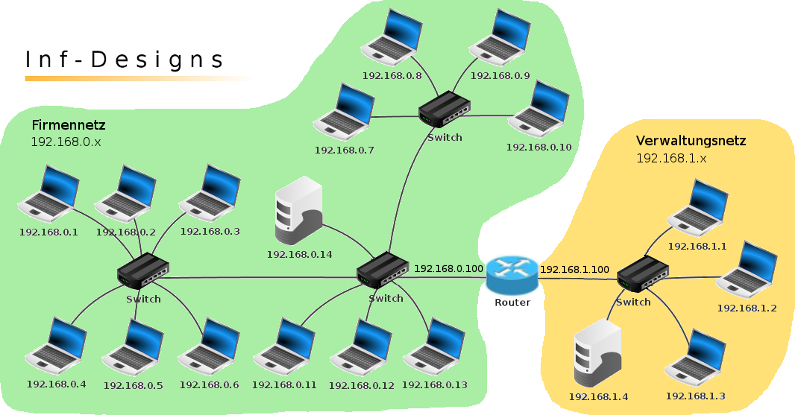
\includegraphics[width=\linewidth]{Grundlagen_Info/07_Netzwerke/Figures/subnets}
    \end{figure}
\end{frame}

\begin{frame}{Netzwerk-Spiel: \textbf{Netzzugangsschicht}}
    \begin{table}[H]
        \centering
        \begin{tabular}{p{2cm}|l}
            \rowcolor{\networkLayerColor!20} Von:                                         & \sout{\texttt{192.168.0.3}}  \\\midrule
            \rowcolor{\networkLayerColor!20} An:                                          & \sout{\texttt{192.168.0.11}} \\\midrule
            \rowcolor{\transportLayerColor!20}Sequenz:                                    & 1                            \\\midrule
            \rowcolor{\applicationLayerColor!20}Nachricht\newline\tiny (max. 10 Zeichen): & \texttt{Hi Bob, wi}          \\
        \end{tabular}
        \begin{tabular}{p{2cm}|l}
            \rowcolor{\networkLayerColor!20} Von:                                         & \sout{\texttt{192.168.0.3}}  \\\midrule
            \rowcolor{\networkLayerColor!20} An:                                          & \sout{\texttt{192.168.0.11}} \\\midrule
            \rowcolor{\transportLayerColor!20}Sequenz:                                    & 2                            \\\midrule
            \rowcolor{\applicationLayerColor!20}Nachricht\newline\tiny (max. 10 Zeichen): & \texttt{e geht's?}           \\
        \end{tabular}
    \end{table}
\end{frame}

\begin{frame}[fragile]{Netzwerk-Spiel: \textbf{Netzzugangsschicht}}{MAC-Adresse}
    \begin{table}[H]
        \footnotesize
        \centering
        \begin{tabular}{l|l}
            \rowcolor{\dataLinkLayerColor!20} Von:         & \texttt{48:2C:6A:1E:59:3D} \\\midrule
            \rowcolor{\dataLinkLayerColor!20} An:          & \texttt{60:4E:46:F5:08:09} \\\midrule
            \rowcolor{\transportLayerColor!20}Sequenz:     & 1                          \\\midrule
            \rowcolor{\applicationLayerColor!20}Nachricht: & \texttt{Hi Bob, wi}        \\
        \end{tabular}
        \begin{tabular}{l|l}
            \rowcolor{\dataLinkLayerColor!20} Von:         & \texttt{48:2C:6A:1E:59:3D} \\\midrule
            \rowcolor{\dataLinkLayerColor!20} An:          & \texttt{60:4E:46:F5:08:09} \\\midrule
            \rowcolor{\transportLayerColor!20}Sequenz:     & 2                          \\\midrule
            \rowcolor{\applicationLayerColor!20}Nachricht: & \texttt{e geht's?}         \\
        \end{tabular}
    \end{table}
    \faFingerprint{} \textbf{MAC-Adresse}
    \begin{itemize}[<+->]
        \item Analogie: Übergabe Brief von einer Hand in die andere
        \item \enquote{Fingerabdruck} eines Computers im Internet
        \item 48 bit, die normalerweise in hexadezimaler Weise angegeben werden
        \item Z.B. \commandbox{48:2C:6A:1E:59:3D}
        \item Jede Netzwerkkarte hat eine MAC-Adresse
    \end{itemize}
\end{frame}

\begin{frame}[fragile]{\faFingerprint{} \acrshort{MAC}-Adresse}{Netzzugangsschicht}
    \begin{center}
        Wie gelangt man überhaupt von einem Computer zum anderen?
    \end{center}
    \begin{itemize}[<+->]
        \item \gls{MAC}-Adresse: In jedem Computer (in Netzwerkkarte) eingebaute Adresse
        \item So etwas wie der \enquote{Fingerabdruck} eines Computers
        \item Analogie: Übergabe Brief von einer Hand in die andere
        \item 48 bit, die normalerweise in hexadezimaler Weise angegeben werden
        \item Z.B. \commandbox{48:2C:6A:1E:59:3D}
    \end{itemize}
\end{frame}

\begin{frame}[fragile]{\acrfull{ARP}}{Verbindungsschicht}
    \begin{itemize}[<+->]
        \item Daten werden zwar mit Ziel-\gls{IP}-Adresse versehen, können jedoch nur von \gls{MAC} zu \gls{MAC} übergeben werden!
        \item Muss verwendet werden, um herauszufinden, welche \gls{MAC}-Adresse zu welcher \gls{IP}-Adresse gehört.
        \item Beispiel
              \begin{itemize}[<+->]
                  \item Computer \commandbox|192.168.0.33| will Nachricht senden an \commandbox|192.168.0.34|, im selben Subnetz!
                  \item \commandbox|192.168.0.33| sendet daher eine Nachricht an alle Computer in \commandbox|192.168.0.x|: \enquote{Wer hat die \gls{IP} \commandbox|192.168.0.34|}?
                  \item Computer \commandbox|192.168.0.34| antwortet: \enquote{Ich! Meine \gls{MAC} ist \commandbox|60:4E:46:F5:08:09|.}
                  \item Nun kann der Computer seine Nachricht an den Empfänger übergeben.
              \end{itemize}
    \end{itemize}
\end{frame}

\begin{frame}{Auftrag (\textasciitilde{} 20')}
    \begin{itemize}
        \item \aufgabebox{1.2-1.4}
        \item \challengebox{1.5}
    \end{itemize}
\end{frame}

\begin{frame}{Topologie, grössere Netzwerke}
    \begin{center}
        Wie bauen wir am besten ein grösseres Netzwerk auf?
    \end{center}

    \begin{figure}[H]
        \centering
        % Bus Topology
        \begin{subfigure}[b]{0.25\textwidth}
            \centering
            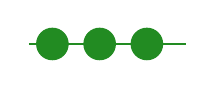
\begin{tikzpicture}
                \draw[ForestGreen, thick] (0,0) -- (2,0); % Bus
                \foreach \x in {0.3, 0.9, 1.5} {
                        \filldraw[ForestGreen] (\x, 0) circle (2mm);
                    }
            \end{tikzpicture}
            \caption{Bus}
        \end{subfigure}%
        % Ring Topology
        \begin{subfigure}[b]{0.25\textwidth}
            \centering
            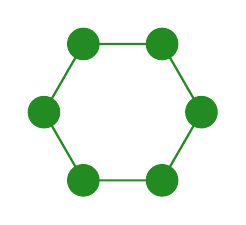
\begin{tikzpicture}
                \draw[ForestGreen, thick] (0:1cm) \foreach \x in {60,120,...,360} {
                        -- (\x:1cm)
                    } -- cycle; % Completes the circle
                \foreach \x in {0,60,...,300} {
                        \filldraw[ForestGreen] (\x:1cm) circle (2mm);
                    }
            \end{tikzpicture}
            \caption{Ring}
        \end{subfigure}
        % Stern
        \begin{subfigure}[b]{0.25\textwidth}
            \centering
            
\begin{tikzpicture}
                \node[fill=ForestGreen, circle, minimum size=5mm] at (0,0) (center) {};
                \foreach \x in {0,45,...,315} {
                        \node[fill=ForestGreen, circle, minimum size=2mm] at (\x:1cm) (node\x) {};
                        \draw[ForestGreen] (center) -- (node\x);
                    }
            \end{tikzpicture}
            \caption{Stern}
        \end{subfigure}%
        % Mesh Topology
        \begin{subfigure}[b]{0.25\textwidth}
            \centering
            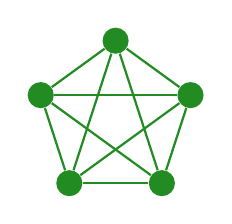
\begin{tikzpicture}
                % Define nodes
                \foreach \x [count=\i from 1] in {18,90,162,234,306} {
                        \node[fill=ForestGreen, circle, minimum size=2mm] at (\x:1cm) (node\i) {};
                    }

                % Connect nodes (to border points)
                \foreach \x in {1,2,3,4,5} {
                        \foreach \y in {\x,...,5} {
                                \ifnum\x=\y\relax
                                    % skip self-connection
                                \else
                                    \draw[ForestGreen, thick] (node\x) -- (node\y);
                                \fi
                            }
                    }

            \end{tikzpicture}
            \caption{Vollvermascht}
        \end{subfigure}
        \begin{subfigure}{.25\textwidth}
            \centering
            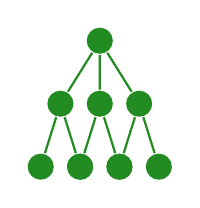
\begin{tikzpicture}[
                    sibling distance=5mm, % Adjust spacing between siblings
                    level distance=8mm, % Adjust spacing between parent and child nodes
                    every node/.style={fill=ForestGreen, circle, thick, minimum size=2mm},
                    edge from parent/.style={ForestGreen, thick, draw}
                ]
                % Define the tree
                \node {} % Root node
                child {node {}
                        child {node {}}
                        child {node {}}
                    }
                child {node {}
                        child {node {}}
                        child {node {}}
                    }
                child {node {}
                        child {node {}}
                        child {node {}}
                    };

            \end{tikzpicture}
            \caption{Baum}
        \end{subfigure}
        \caption{Beispiele von Netzwerk-Topologien}
        \label{fig:topologie}
    \end{figure}

\end{frame}

\begin{frame}{Unicast, Broadcast, Multicast}
    \begin{itemize}
        \item \textbf{Unicast}: Nachricht wird an einen einzigen Empfänger gesendet
        \item \textbf{Broadcast}: Nachricht wird an alle Empfänger im selben Subnetz gesendet
        \item \textbf{Multicast}: Nachricht wird an eine ausgewählte Gruppe von Empfängern gesendet
    \end{itemize}
    \begin{figure}[H]
        \centering
        % Use three responsive subfigures that scale to the local \linewidth so they look good
        % both in beamer (narrow) and article (wide).
        \begin{subfigure}[b]{0.32\linewidth}
            \centering
            \resizebox{\linewidth}{!}{%
                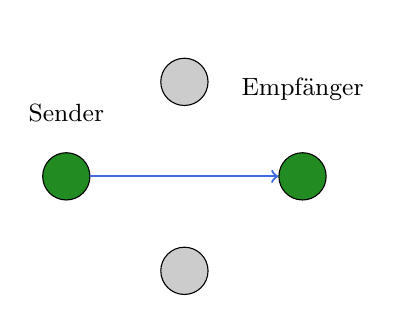
\begin{tikzpicture}[every node/.style={circle,minimum size=6mm,inner sep=0pt}]
                    % Nodes
                    \node[fill=ForestGreen, draw=black] (A) at (0,0) {};
                    \node[fill=ForestGreen, draw=black] (B) at (3,0) {};
                    \node[fill=Gray!40, draw=black] (C) at (1.5,1.2) {};
                    \node[fill=Gray!40, draw=black] (D) at (1.5,-1.2) {};
                    % Labels
                    \node[above,font=\small] at (A.north) {Sender};
                    \node[above,font=\small] at (B.north) {Empfänger};
                    % Arrow
                    \draw[->, thick, RoyalBlue] (A) -- (B);
                \end{tikzpicture}%
            }
            \caption*{\small Unicast: \texttt{1:1}}
        \end{subfigure}\pause\hfill
        \begin{subfigure}[b]{0.32\linewidth}
            \centering
            \resizebox{\linewidth}{!}{%
                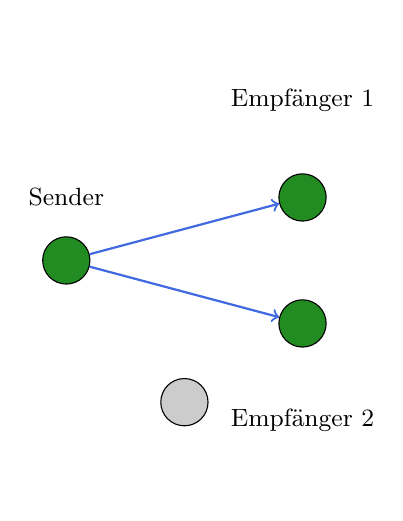
\begin{tikzpicture}[every node/.style={circle,minimum size=6mm,inner sep=0pt}]
                    % Nodes
                    \node[fill=ForestGreen, draw=black] (A) at (0,0) {};
                    \node[fill=ForestGreen, draw=black] (B) at (3,0.8) {};
                    \node[fill=ForestGreen, draw=black] (C) at (3,-0.8) {};
                    \node[fill=Gray!40, draw=black] (D) at (1.5,-1.8) {};
                    % Labels
                    \node[above,font=\small] at (A.north) {Sender};
                    \node[above,font=\small] at (B.north) {Empfänger 1};
                    \node[below,font=\small] at (C.south) {Empfänger 2};
                    % Arrows
                    \draw[->, thick, RoyalBlue] (A) -- (B);
                    \draw[->, thick, RoyalBlue] (A) -- (C);
                \end{tikzpicture}%
            }
            \caption*{\small Multicast: \texttt{1:n}}
        \end{subfigure}\pause\hfill
        \begin{subfigure}[b]{0.32\linewidth}
            \centering
            \resizebox{\linewidth}{!}{%
                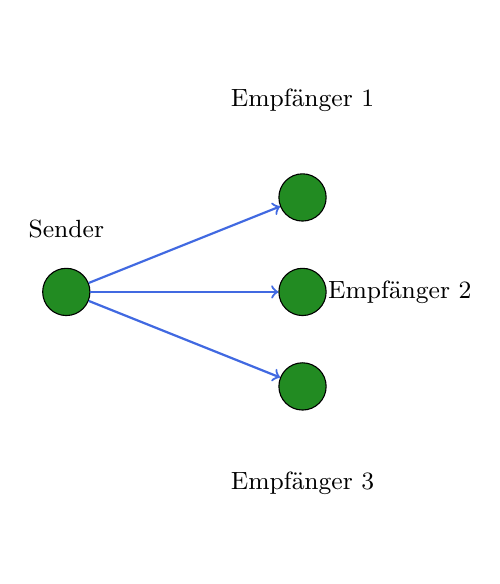
\begin{tikzpicture}[every node/.style={circle,minimum size=6mm,inner sep=0pt}]
                    % Nodes
                    \node[fill=ForestGreen, draw=black] (A) at (0,0) {};
                    \node[fill=ForestGreen, draw=black] (B) at (3,1.2) {};
                    \node[fill=ForestGreen, draw=black] (C) at (3,0) {};
                    \node[fill=ForestGreen, draw=black] (D) at (3,-1.2) {};
                    % Labels
                    \node[above,font=\small] at (A.north) {Sender};
                    \node[above,font=\small] at (B.north) {Empfänger 1};
                    \node[right,font=\small] at (C.east) {Empfänger 2};
                    \node[below,font=\small] at (D.south) {Empfänger 3};
                    % Arrows
                    \draw[->, thick, RoyalBlue] (A) -- (B);
                    \draw[->, thick, RoyalBlue] (A) -- (C);
                    \draw[->, thick, RoyalBlue] (A) -- (D);
                \end{tikzpicture}%
            }
            \caption*{\small Broadcast: \texttt{1:alle}}
        \end{subfigure}
    \end{figure}
\end{frame}

\begin{frame}{Auftrag (\textasciitilde{} 10')}
    \begin{itemize}
        \item \aufgabebox{1.7-1.10}
    \end{itemize}
\end{frame}



\section{Vermittlungsschicht}
\setbeamercolor{frametitle}{bg=\networkLayerColor!20}

\begin{frame}[fragile]{\faMapMarker{} \gls{IP}-Adresse}{Vermittlungsschicht}

    \begin{itemize}[<+->]
        \item \gls{IP}-Adresse = Netzwerk-Adresse eines Computers
        \item Analogie: Wohnadresse einer Person (Strasse \& Stadt)
        \item Häufig im \gls{IP}v4-Format: 4 bytes, also 4 Zahlen von 0-255, z.B.:\\
              \textcolor{blue}{\texttt{11000000.10101000.00000001.00000101}}
        \item Wird meist dezimal angegeben, z.B. \textcolor{blue}{\texttt{192.168.1.5}}

        \item Wie viele \gls{IP}v4-Adressen gibt es? Reicht das?
              \begin{itemize}
                  \item $4\cdot 8 \text{ bits} = 32 \text{ bits}$
                        \[2^{32} \sim 4 \text{ Milliarden Adressen} \rightarrow \text{zu wenig!}\]
              \end{itemize}
        \item \gls{IP}v6: 128 bits, fast unendlich viele Adressen
              \[2^{128} \sim 3.4\cdot 10^{38}  \text{ Adressen}\]
    \end{itemize}
\end{frame}

\begin{frame}{\faMapMarker{} \gls{IP}-Adresse}{Lokale und globale Adressen}
    \textbf{Lokale} vs. \textbf{globale} \gls{IP}-Adresse
    \begin{itemize}
        \item Aufgrund von \gls{IP}v4-Mangel: Unterscheidung zwischen lokalen und globalen \gls{IP}-Adressen
        \item \textbf{Lokale \gls{IP}}: nur im lokalen Netzwerk gültig (z.B. 192.168.x.x, 10.x.x.x)
        \item \textbf{Globale \gls{IP}}: weltweit eindeutig (z.B. 8.8.8.8)
    \end{itemize}
\end{frame}

\begin{frame}[fragile]{Lokale vs. globale \gls{IP}-Adresse}{\acrfull{NAT}}
    \begin{figure}[H]
        \centering
        \resizebox{\linewidth}{!}{
            \begin{tikzpicture}[
                    base/.style={rectangle, draw, minimum width=2.5cm, minimum height=1cm, text=white, rounded corners, text width=2.5cm, align=center, inner sep=8pt},
                    device/.style={base, fill=ForestGreen},
                    router/.style={base, fill=\networkLayerColor},
                    server/.style={base, fill=Crimson},
                    arrow/.style={-Stealth, thick, text width=3cm, align=center}
                ]

                % Nodes
                \node[device] (client) {Client\\\texttt{192.168.0.10}};
                \node[device, below=.5cm of client] (client2) {Client\\\texttt{192.168.0.11}};
                \node[device, below=.5cm of client2] (client3) {Client\\\texttt{192.168.0.12}};
                \node[router, right=3cm of client2] (nat) {Router\\\texttt{80.152.43.21}};
                \node[server, right=3cm of nat] (web) {Webserver\\\texttt{159.233.1.22}};

                \node[draw=Crimson!60, rounded corners, thick, dashed, inner sep=6pt, fit=(client)(client2)(client3)(nat)] (lan2area){};

                % Label boxes
                \node[red, align=left, font=\small, anchor=south west] at (lan2area.north west) {Lokales Netzwerk};
                \node[below=0.5cm of web, text width=2.5cm, align=center, font=\small] {Internet};

                % Arrows and animations
                \only<1>{
                    \draw[arrow] (client.east) -- (nat.west) node[midway, above, text=black] {Anfrage von\\\texttt{192.168.0.10}};
                }
                
                \only<2>{
                    \draw[arrow] (nat.east) -- (web.west) node[midway, above, text=black] {Anfrage von\\\texttt{80.152.43.21} \faCheck};
                }
                
                \only<3>{
                    \draw[arrow] (web.west) -- (nat.east) node[midway, below, text=black] {Antwort an\\\texttt{80.152.43.21}};
                }
                
                \only<4>{
                    \draw[arrow] (nat.west) -- (client.east) node[midway, below, text=black] {Antwort an\\\texttt{192.168.0.10} \faCheck};
                }

                % NAT table
                \only<2->{
                    \node[below=0.1cm of nat, text width=3.5cm, font=\tiny, inner sep=8pt, draw, rounded corners, fill=\networkLayerColor!10] (natTable) {
                        \textbf{\acrshort{NAT}-Tabelle}
                        \begin{tabular}{p{1.4cm}|p{1.4cm}}
                            \textbf{Lokal} & \textbf{Global} \\
                            \midrule\midrule
                            192.168.0.10 & 80.152.43.21 \\

                        \end{tabular}
                    };
                }
            \end{tikzpicture}
        }
    \end{figure}
    
    \only<1-2>{
        \textbf{Ausgehende Anfrage}
        \begin{itemize}
            \item Client sendet Anfrage mit lokaler IP-Adresse
            \item Router ersetzt lokale IP durch seine globale IP
        \end{itemize}
    }
    
    \only<3-4>{
        \textbf{Eingehende Antwort}
        \begin{itemize}
            \item Server antwortet an die globale IP des Routers
            \item Router schlägt in NAT-Tabelle nach und leitet an lokale IP weiter
        \end{itemize}
    }
\end{frame}

\begin{frame}[fragile]{Eigene IP-Adresse herausfinden}
    \begin{itemize}
        \item MacOS, Terminal (via Spotlight-Suche): \\
              \commandbox*|ipconfig getifaddr en0|
        \item Windows, Programm \enquote{\texttt{cmd}} (via \keys{\faWindows + R}): \\
              \commandbox*|ipconfig|
    \end{itemize}
\end{frame}

\begin{frame}[fragile]{\faCompass{} \texttt{ping}}{Vermittlungsschicht}

    \begin{itemize}[<+->]
        \item Im Terminal / cmd: \commandbox*|ping [ip address]|, z.B.:\\
              \commandbox*|ping 159.233.1.22|
        \item Minimale Nachricht an andere \gls{IP}-Adresse schicken
        \item Ziel: schauen ob eine \gls{IP} existiert, bzw. erreichbar ist, wird mittels \gls{ICMP} realisiert
    \end{itemize}
\end{frame}

\begin{frame}
    Auftrag
    \begin{itemize}
        \item \aufgabebox{1.11 - 1.13}: eigene IPv4-Adresse herausfinden
        \item \aufgabebox{1.15 - 1.17}: Notation \gls{IP}v4 und \gls{IP}v6
        \item \challengebox{1.14}: \acrshort{ARP}-Scan
    \end{itemize}
\end{frame}

\begin{frame}[fragile]{\faMapMarker{} Sub-Netze}{Vermittlungsschicht}
    \begin{figure}[H]
        \centering
        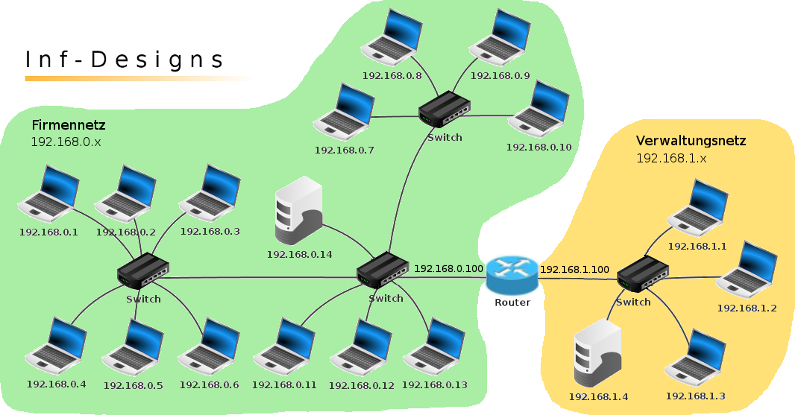
\includegraphics[width=\linewidth]{Grundlagen_Info/07_Netzwerke/Figures/subnets}
    \end{figure}
\end{frame}

\begin{frame}[fragile]{\faMapMarker{} Sub-Netze}{Vermittlungsschicht}
    \begin{center}
        \textbf{Switch} oder \textbf{Router}?!?
    \end{center}
    \begin{figure}[H]
        \centering
        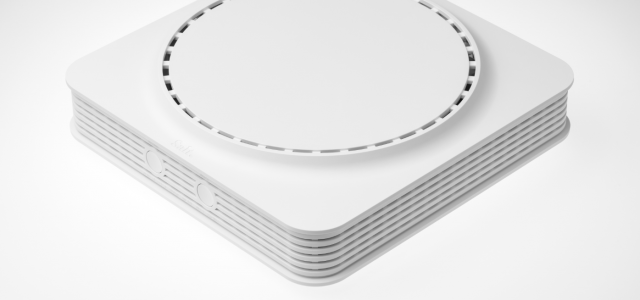
\includegraphics[width=0.38\linewidth]{Grundlagen_Info/07_Netzwerke/Figures/salt}
        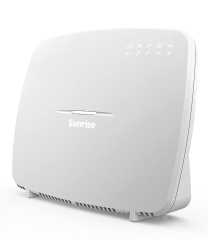
\includegraphics[width=0.2\linewidth]{Grundlagen_Info/07_Netzwerke/Figures/sunrise}
        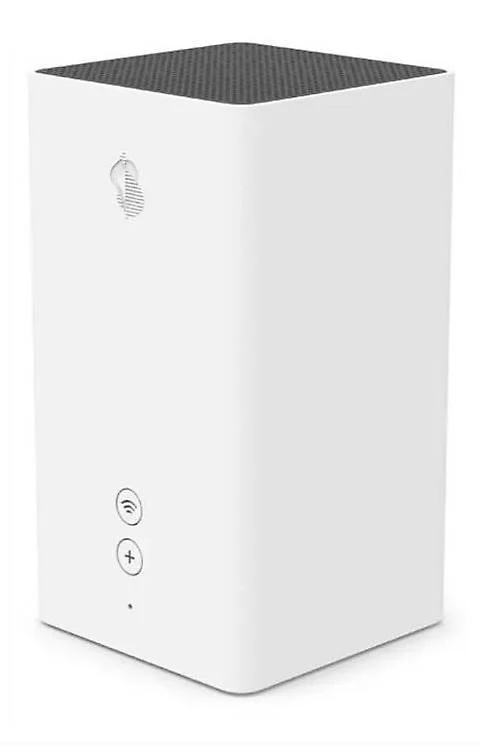
\includegraphics[width=0.2\linewidth]{Grundlagen_Info/07_Netzwerke/Figures/swisscom}
    \end{figure}
\end{frame}

\begin{frame}[fragile]{\faMapMarker{} Sub-Netze}{Vermittlungsschicht}
    \begin{center}
        \textbf{Switch} oder \textbf{Router}?!?
    \end{center}
    \begin{figure}[H]
        \centering
        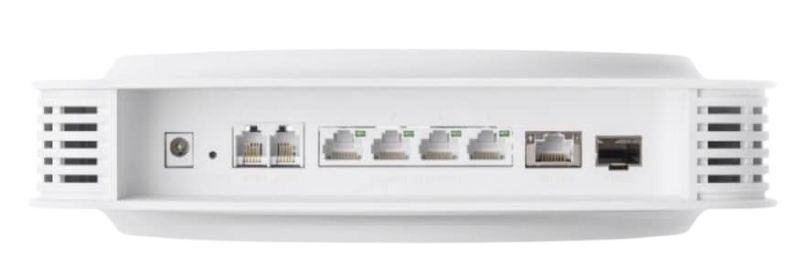
\includegraphics[width=0.38\linewidth]{Grundlagen_Info/07_Netzwerke/Figures/salt-back}
        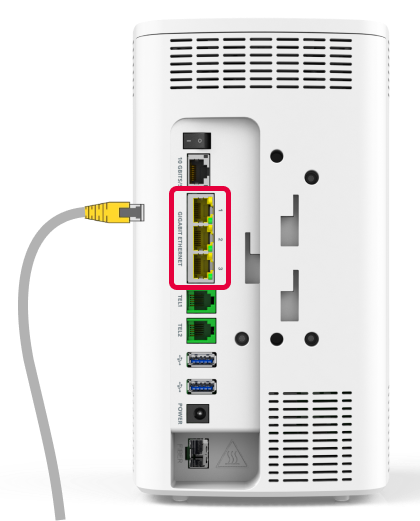
\includegraphics[width=0.2\linewidth]{Grundlagen_Info/07_Netzwerke/Figures/sunrise-back}
        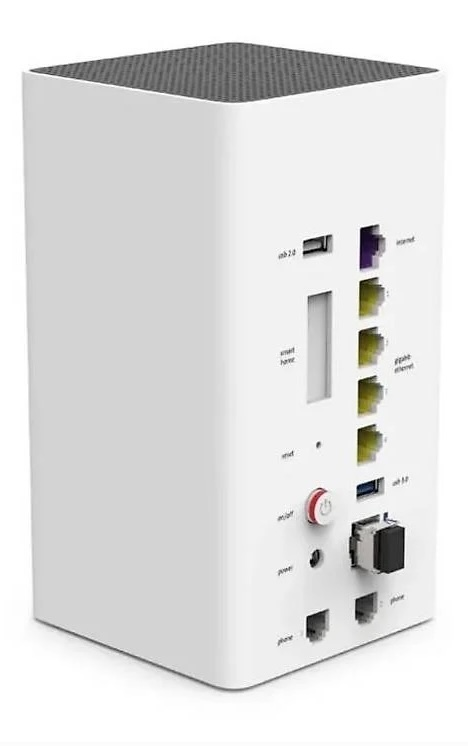
\includegraphics[width=0.2\linewidth]{Grundlagen_Info/07_Netzwerke/Figures/swisscom-back}
    \end{figure}
    \pause
    \begin{center}
        Beides (meistens) im gleichen Gerät!
    \end{center}
\end{frame}

\begin{frame}[fragile]{\faMapMarker{} Sub-Netze}{Vermittlungsschicht}
    \textbf{Subnetzwerke}
    \begin{itemize}[<+->]
        \item Verschiedene Geräte gehören zum gleichen Subnetz, falls Sie
              \begin{itemize}
                  \item Physisch miteinander verbunden sind (WLAN, Kabel, etc.)
                  \item Die gleiche Subnetzmaske teilen (später mehr dazu)
              \end{itemize}
    \end{itemize}
\end{frame}

\begin{frame}[fragile]{\faGlobe{} Netzmasken}{Vermittlungsschicht}
    \textbf{Netzmaske}
    \begin{itemize}[<+->]
        \item Sieht ähnlich aus wie eine IP-Adresse: \commandBluebox|xxx.xxx.xxx.xxx|
        \item Fasst mehrere IPs zu einer Gruppe (= Subnetz) zusammen
        \item Gibt an, wie viele Stellen einer IP-Adresse gleich sein müssen, damit mehrer Computer zum gleichen (Sub-)Netzwerk gehören.
        \item \textbf{Beispiel}:
              \begin{table}[H]
                  \centering
                  \tiny
                  \begin{tabular}{r|l|l}
                                   & Dezimal                        & Binär                                                                 \\\midrule\midrule
                      IP 1         & \texttt{159.233.1.22}          & \texttt{\textcolor{ForestGreen}{10011111.11101001.00000001}.00010110} \\\midrule
                      IP 2         & \texttt{159.233.1.1}           & \texttt{\textcolor{ForestGreen}{10011111.11101001.00000001}.00000001} \\\midrule
                      Subnetzmaske & \commandBluebox|255.255.255.0| & \texttt{\textcolor{ForestGreen}{11111111.11111111.11111111}.00000000}
                  \end{tabular}
              \end{table}
              Bedeutet, dass alle IP-Adressen die mit \commandbox|159.233.1.[...]| anfangen, zum selben Netzwerk gehören
        \item Wird manchmal \enquote{informell} auch so angegeben: \commandBluebox|159.233.1.x|
    \end{itemize}
\end{frame}

\begin{frame}[fragile]{Subnetze \& Netzmasken}{Übung}
    \begin{table}[H]
        \centering
        \footnotesize
        \begin{tabular}{l|l|l|p{2cm}}

            \textbf{Eigene IP} & \textbf{Netzmaske} & \textbf{Ziel-IP} & \textbf{Gleiches \newline Subnetz?} \\\midrule\midrule

            213.45.19.89       & 255.255.255.0      & 213.45.17.89     &                                     \\\midrule

            213.45.19.89       & 255.255.0.0        & 213.45.17.89     &                                     \\\midrule

            88.100.11.17       & 255.255.255.0      & 88.100.11.254    &                                     \\\midrule

            88.100.11.17       & 0.0.0.0            & 213.45.19.89     &                                     \\\midrule

            10.0.0.0           & 255.255.255.252    & 10.0.0.1         &                                     \\\midrule
            1.2.3.0            & 255.255.255.252    & 1.2.3.5          &
        \end{tabular}
    \end{table}
    \begin{itemize}
        \item $\rightarrow$ IPs dürfen sich nur an denjenigen Stellen unterscheiden, wo in der Maske (binär!) Nullen stehen.
        \item Umrechner dezimal $\rightarrow$ binär: \qrcode[height=1cm]{https://oinf.ch/interactive/ips-und-netzmaske/}
    \end{itemize}
\end{frame}

\begin{frame}[fragile]{Subnetze \& Netzmasken}{Aufträge (Skript)}
    \begin{itemize}
        \item Subnetzmasken
              \begin{itemize}
                  \item \aufgabebox{Netzmasken: 1.20-1.23}
                  \item \aufgabebox{Filius: 1.24}
                  \item \challengebox{1.25}
              \end{itemize}
    \end{itemize}
\end{frame}

\begin{frame}[fragile]{Subnetze \& Netzmasken}{Weitere Übungen (Lösung)}
    \begin{table}[H]
        \centering
        \resizebox{\textwidth}{!}{
            \begin{tabular}{p{1.2cm}||c|c||c|c||c|c|}
                \textbf{Netzmaske Subnetz} & \multicolumn{2}{c||}{255.255.255.0} & \multicolumn{2}{c||}{255.255.0.0} & \multicolumn{2}{c|}{255.255.255.240}                                        \\
                \cmidrule{2-7}
                                           & IP 3.4.5.6                          & IP 3.3.3.3                        & IP 3.4.5.6                           & IP 3.3.3.3 & IP 3.4.5.6 & IP 3.3.3.3 \\
                \midrule\midrule
                3.3.3.4                    & Nein                                & Ja                                & Nein                                 & Ja         & Nein       & Ja         \\\midrule
                4.4.4.3                    & Nein                                & Nein                              & Nein                                 & Nein       & Nein       & Nein       \\\midrule
                3.4.5.99                   & Ja                                  & Nein                              & Ja                                   & Nein       & Nein       & Nein       \\\midrule
                3.3.4.4                    & Nein                                & Nein                              & Nein                                 & Ja         & Nein       & Nein       \\\midrule
                3.4.7.7                    & Nein                                & Ja                                & Ja                                   & Nein       & Nein       & Nein       \\\midrule
                3.3.3.17                   & Nein                                & Ja                                & Nein                                 & Ja         & Nein       & Nein       \\
            \end{tabular}}
    \end{table}
\end{frame}

\section{Transportschicht}
\setbeamercolor{frametitle}{bg=\transportLayerColor!20}

\begin{frame}{Netzwerk-Spiel: \textbf{Transportschicht}}
    Endgeräte trennen die Nachrichten in Segmente auf und fügen Sequenznummern hinzu:
    \begin{table}[H]
        \centering

        \begin{tabular}{p{2cm}|l}
            \rowcolor{\transportLayerColor!20}Sequenz:                                    & 1                   \\\midrule
            \rowcolor{\applicationLayerColor!20}Nachricht\newline\tiny (max. 10 Zeichen): & \texttt{Hi Bob, wi} \\
        \end{tabular}
        \begin{tabular}{p{2cm}|l}
            \rowcolor{\transportLayerColor!20}Sequenz:                                    & 2                  \\\midrule
            \rowcolor{\applicationLayerColor!20}Nachricht\newline\tiny (max. 10 Zeichen): & \texttt{e geht's?} \\
        \end{tabular}
    \end{table}
\end{frame}

\begin{frame}[fragile]{\faBoxOpen{} TCP (\textit{Transmission Control Protocol}) Header}{Transportschicht}
    TCP = Übertragungssteuerungsprotokoll
    \begin{table}[H]
        \centering
        \begin{tabular}{>{\raggedright\arraybackslash}p{4cm}|>{\raggedright\arraybackslash}p{4cm}}

		\rowcolor{\transportLayerColor!30}\multicolumn{2}{c}{\textbf{\gls{TCP} Header}}       \\ \midrule\midrule
		\rowcolor{\transportLayerColor!15}Source Port & Destination Port                      \\ \midrule
		\rowcolor{\transportLayerColor!15}\multicolumn{2}{c}{Sequence \# (SEQ)}               \\ \midrule
		\rowcolor{\transportLayerColor!15}\multicolumn{2}{c}{Acknowledgement \# (ACK)}        \\ \midrule
		\rowcolor{\transportLayerColor!15}\multicolumn{2}{c}{Weitere \gls{TCP}-Header-Felder} \\ \midrule
		\rowcolor{orange!30}\multicolumn{2}{c}{\textbf{Nutzdaten}}                            \\ \midrule\midrule
		\rowcolor{orange!15}\multicolumn{2}{c}{$\ldots$ Anwendungsdaten $\ldots$}             \\
	\end{tabular}
    \end{table}
\end{frame}

\begin{frame}[fragile]{\faShip{} Ports}{Transportschicht}
    \begin{table}[H]
        \centering
        \begin{tabular}{ccc}
            \toprule
            \textbf{Portnummer} & \textbf{Anwendung} & \textbf{Verwendung}             \\
            \midrule
            20                  & FTP                & Dateitransfer                   \\
            21                  & FTP                & Befehlssteuerung                \\
            22                  & SSH                & Sichere Shell-Zugriffe          \\
            23                  & Telnet             & Unverschlüsselte Fernsteuerung  \\
            25                  & SMTP               & E-Mail-Versand                  \\
            53                  & DNS                & Namensauflösung                 \\
            80                  & HTTP               & Webseiten-Abruf                 \\
            110                 & POP3               & E-Mail-Abholung                 \\
            143                 & IMAP               & E-Mail-Management               \\
            443                 & HTTPS              & Verschlüsselter Webseiten-Abruf \\
            993                 & IMAP               & E-Mail-Management über SSL      \\
            995                 & POP3               & E-Mail-Abholung über SSL        \\
            \bottomrule
        \end{tabular}
        \caption*{Gängige TCP-Ports, Anwendungen und deren Verwendung}
    \end{table}
\end{frame}

\begin{frame}[fragile]{\faHandshake{} TCP: 3-way handshake}{Transportschicht}
    \begin{columns}[c]
        \begin{column}{.6\textwidth}
            \begin{figure}[H]
                \centering
                \begin{tikzpicture}[>=Stealth, font=\sffamily, node distance=2cm and 4cm]
                    % Draw the entities
                    \tikzset{c/.append style={fill=\networkLayerColor!30,rounded corners,above, align=center, text width=3cm}}
                    \tikzset{person/.append style={text width=1.2cm,fill=ForestGreen!30,rounded corners,align=center}}
                    \node[person](Bob) {\tiny \faMale{} Bob\\\texttt{10.0.0.2:21}};
                    \node[person, right=of Bob] (Alice) {\tiny \faFemale{} Alice\\\texttt{10.0.0.3:21}};


                    \node[below of=Bob, yshift=-3.5cm] (BobZeit) {Zeit};
                    \node[below of=Alice, yshift=-3.5cm] (AliceZeit) {Zeit};

                    % Time line
                    \draw[->, thick] (Bob.south) -- node[xshift=-.2cm, rotate=270] {Zeitachse von Bob} (BobZeit);
                    \draw[->, thick] (Alice.south) -- node[xshift=.2cm, rotate=270] {Zeitachse von Alice} (AliceZeit);

                    % Draw the arrows and labels
                    \draw[->, thick, red, dashed] (Bob.south) -- node[c] {\tiny Ich möchte mit dir sprechen, Alice, auf Port 21. Bist du offen?\\SYN=1, SEQ\# 10} ([yshift=-1.5cm]Alice.south);

                    \only<2->{
                        \draw[->, thick, red, dashed] ([yshift=-1.5cm]Alice.south) -- node[c] {\tiny Ok, lass uns reden Bob! Ich bin offen auf Port 21.\\SYN=1, ACK=1, ACK=11} ([yshift=-3cm]Bob.south);
                    }

                    \only<3->{
                        \draw[->, thick, red, dashed] ([yshift=-3cm]Bob.south) -- node[c] {\tiny Ok, danke Alice.\\ACK=1, SEQ\#11} ([yshift=-4.5cm]Alice.south);
                    }
                \end{tikzpicture}
            \end{figure}
        \end{column}\vrule{}
        \begin{column}{.4\textwidth}
            \footnotesize
            \begin{enumerate}
                \item Computer A (\textit{client}, \texttt{10.0.0.2}) erstellt eine Verbindungsanfrage zum Computer B (\textit{server}, \texttt{10.0.0.3}), mittels einem Paket, das nur das \texttt{SYN}-Flaggen gesetzt hat.
                \item Der Server antwortet sowohl mit einem gesetzten \texttt{SYN} und einem \texttt{ACK}-Flaggen
                \item Im letzten Schritt antwortet der \textit{client} nochmals mit einem einzelnen \texttt{ACK}-Flaggen\\
                      $\rightarrow$ TCP-Verbindung ist nun erstellt!
            \end{enumerate}
        \end{column}
    \end{columns}
\end{frame}

\begin{frame}[fragile]{\faHandshake{} TCP: 3-way handshake}{Auftrag}
    \begin{itemize}
        \item Skript: \aufgabebox{1.28-1.29}
    \end{itemize}
\end{frame}


\section{Anwendungsschicht}
\setbeamercolor{frametitle}{bg=\applicationLayerColor!20}

\begin{frame}{Netzwerk-Spiel: \textbf{Anwendungsschicht}}
    Endgeräte verfassen Nachrichten:
    \begin{table}[H]
        \centering
        \begin{tabular}{p{2cm}|l}
            \rowcolor{\applicationLayerColor!20}Nachricht\newline\tiny (max. 10 Zeichen): & \texttt{Hi Bob, wi} \\
        \end{tabular}
        \begin{tabular}{p{2cm}|l}
            \rowcolor{\applicationLayerColor!20}Nachricht\newline\tiny (max. 10 Zeichen): & \texttt{e geht's?} \\
        \end{tabular}
    \end{table}
\end{frame}


\begin{frame}[fragile]{Webserver}
    \begin{figure}[H]
        \centering
        \resizebox{\linewidth}{!}{
            \begin{tikzpicture}[
                    font=\sffamily,
                    every node/.style={align=center},
                    entity/.style={rectangle, draw, fill=\networkLayerColor, text=white, minimum height=2.5cm, minimum width=3cm, rounded corners, text width=2.3cm, align=center, node distance=1.5cm and 6.5cm},
                    process/.style={-Stealth, thick, draw},
                    arrowtext/.style={text width=5.5cm, align=center, text=black, font=\footnotesize}
                ]

                % nodes for client
                \node[entity] (clientStart) {Eingabe der \acrshort{URL} am Bildschirm};
                \node[entity, below=of clientStart] (clientEnd) {Sammelt Daten, setzt Website zusammen (Darstellung)};
                % Draw a 2D rectangle around the users
                \node[fit=(clientStart) (clientEnd), inner sep=4pt, red, text=black, dotted, draw, line width=1pt,rounded corners](browser) {Client\\ \faLaptop};

                % nodes for server
                \node[entity, right=of clientStart] (serverStart) {Interpretiert die Anfrage und sucht die Dateien};
                \node[entity, right=of clientEnd] (serverEnd) {Sendet den Status der Suche und die Dateien der Webseite};
                % Draw a 2D rectangle around the users
                \node[fit=(serverStart) (serverEnd), inner sep=4pt, red, text=black, dotted, draw, line width=1pt,rounded corners](server) {Web Server\\ \faServer};

                % Connections
                \draw[process, Crimson] (clientStart.east) -- node[arrowtext, above] {\texttt{http://192.168.10.2/index.html}\\(HTTP-Anfrage \texttt{GET /index.html})} (serverStart.west);
                \draw[process, ForestGreen] (serverEnd.west) -- node[arrowtext, below] {HTTP-Antwort \\(Statuscode + Daten)} (clientEnd.east);
            \end{tikzpicture}
        }
        \caption{Schematischer Ablauf eines Webseiten-Aufrufs mit dem \gls{HTTP}-Protokoll}
        \label{fig:http-request-simple}
    \end{figure}
\end{frame}

\begin{frame}[fragile]{\faLaptop{} Client vs Server vs Host}{Anwendungsschicht}
    Definitionen
    \begin{itemize}[<+->]
        \item \textbf{Client}
              \begin{itemize}
                  \item \enquote{Kunde} (von en. \textit{client})
                  \item Computer(-Programm), das etwas will
              \end{itemize}
        \item \textbf{Server}
              \begin{itemize}
                  \item \enquote{Diener} (von en. \textit{to serve} = bedienen, $\neq$ \enquote{surf})
                  \item Computer(-Programm), das etwas hat, das andere Computer(-Programme) brauchen
                  \item Kann Verbindungsanfragen von anderen Computer(-Programmen) akzeptieren / ablehnen
              \end{itemize}
        \item \textbf{Host}
              \begin{itemize}
                  \item = Computer in einem Netzwerk, allgemein für \enquote{server} oder \enquote{client}
                  \item \textit{Host name} = Name eines Computers
              \end{itemize}

    \end{itemize}
\end{frame}

\begin{frame}[fragile]{\faSafari{} Browser}{Anwendungsschicht}
    \begin{itemize}
        \item Browser = Programm, kann eine Datei (meist \texttt{.html})...
              \begin{itemize}
                  \item ...über das Internet \textit{anfordern}
                  \item ...nach dem Empfang \textit{darstellen}
              \end{itemize}
        \item Das Senden / Empfangen von Dateien übernimmt das Betriebssystem (z.B. Windows, MacOS)
        \item Beispiele:
              \begin{itemize}
                  \item \faChrome{} Chrome
                  \item \faFirefox{} Firefox
                  \item \faSafari{} Safari
                  \item \faEdge{} Edge
                  \item  etc.
              \end{itemize}
    \end{itemize}
\end{frame}


\begin{frame}[fragile]{\faSitemap{} URL (Uniform Resource Locator)}{Präsentationsschicht: Webseiten}

    URL = Web-Adresse

    \[
        \underbrace{\text{http://}}_{\text{Protokoll}}
        \underbrace{\text{www.}}_{\text{Server}}
        \underbrace{\text{beispiel.}}_{\text{Domain}}
        \underbrace{\text{ch}}_{\text{TLD\tikzmark{tld}}}
        \underbrace{\text{/dokumente/}}_{\text{Ordner}}
        \underbrace{\text{reglemente.html}}_{\text{Dateiname}}
    \]
    \begin{tikzpicture}[overlay, remember picture]
        \node[below=of tld] (tldFull) {Top Level Domain};
        \draw[red,-stealth] (tld.north) to[bend right] (tldFull);
    \end{tikzpicture}

    \begin{itemize}[<+->]
        \item Erster Teil bezeichnet einen \textit{Server}
              \begin{itemize}
                  \item z.B. 58.55.110.9 $\rightarrow$ \texttt{www.beispiel.ch}
              \end{itemize}
        \item Alles nach der TLD ist ein normaler Ordnerpfad auf dem Computer
    \end{itemize}

\end{frame}

\begin{frame}[fragile]{\faServer{} HTTP(S)-Protokoll}
    \begin{figure}[H]
        \centering
        \resizebox{\linewidth}{!}{
            \begin{tikzpicture}[
                    font=\sffamily,
                    every node/.style={align=center},
                    entity/.style={rectangle, draw, fill=\networkLayerColor, text=white, minimum height=2.5cm, minimum width=3cm, rounded corners, text width=2.3cm, align=center, node distance=1.5cm and 3.5cm},
                    process/.style={-Stealth, thick, draw},
                    arrowtext/.style={text width=2.5cm, align=center, text=black, font=\footnotesize}
                ]

                % Nodes for user
                \node[entity] (userStart) {Eingabe der \acrshort{URL} am Bildschirm};
                \node[entity, below=of userStart] (userEnd) {Webseite am Bildschirm};
                % Draw a 2D rectangle around the users
                \node[fit=(userStart) (userEnd), inner sep=4pt, red, text=black, dotted, draw, line width=1pt,rounded corners](user) {User \\ \faUser};

                % nodes for 
                \node[entity, right=of userStart] (browserStart) {Übersetzt die URL in einen HTTP-Request};
                \node[entity, right=of userEnd] (browserEnd) {Sammelt Daten, setzt Website zusammen (rendern)};
                % Draw a 2D rectangle around the users
                \node[fit=(browserStart) (browserEnd), inner sep=4pt, red, text=black, dotted, draw, line width=1pt,rounded corners](browser) {Browser\\ \faLaptop};

                % nodes for server
                \node[entity, right=of browserStart] (serverStart) {Interpretiert den Request und sucht die Dateien};
                \node[entity, right=of browserEnd] (serverEnd) {Sendet den Status der Suche und die Daten zur Webseite};
                % Draw a 2D rectangle around the users
                \node[fit=(serverStart) (serverEnd), inner sep=4pt, red, text=black, dotted, draw, line width=1pt,rounded corners](server) {Web Server\\ \faServer};

                % Connections
                \draw[process, Crimson] (userStart.east) -- node[arrowtext, above] {1. URL \\ \texttt{http://\\www.beispiel.ch/\\index.html}} (browserStart.west);
                \draw[process, Crimson] (browserStart.east) -- node[arrowtext, above] {2. HTTP Request \\ \texttt{GET /index.html}} (serverStart.west);
                \draw[process, ForestGreen] (serverEnd.west) -- node[arrowtext, below] {3. HTTP Response \\ Statuscode + Daten} (browserEnd.east);
                \draw[process, ForestGreen] (browserEnd.west) -- node[arrowtext, below] {4. Webpage \\ Darstellung der Webseite \texttt{index.html}} (userEnd.east);

            \end{tikzpicture}}
    \end{figure}
\end{frame}



\begin{frame}[fragile]{\faLaptop{} Webseiten}{Präsentationsschicht}
    Beispiel: HTML (\textit{Hypertext Markup Language})
    \begin{itemize}[<+->]
        \item Demo (\textit{Inspect Element} oder \textit{View Page Source})
        \item Speichert die Struktur einer Webseite
        \item Kann weitere Dateien enthalten, beispielsweise:
              \begin{itemize}
                  \item CSS (Cascading Style Sheet), für die Darstellung (Farbe, Grösse etc.)
                  \item JavaScript, jQuery etc. für die Interaktivität (Ein- und Ausblenden von Objekten etc.)
              \end{itemize}
        \item Wie man eine Webseite baut ist hier nicht das Hauptthema, wird aber in der Interessenwoche vermittelt
    \end{itemize}
\end{frame}

\begin{frame}[fragile]{Webserver}{Aufträge (Skript)}
    \begin{itemize}
        \item \aufgabebox{Filius (Echo-Server): 1.30}
        \item \aufgabebox{Filius (Email-Server): 1.31}
        \item \aufgabebox{Filius (Web-Server): 1.32}
    \end{itemize}
\end{frame}



\begin{frame}[fragile]{\acrfull{DNS}}
    \begin{itemize}
        \item Wenn Sie auf eine Webseite wie \url{https://sbb.ch} gehen, woher weiss der Client, von welchem Server er die Informationen anfragen soll?
        \item \gls{DNS}: \acrshort{URL} $\rightleftarrows$ \acrshort{IP}-Adresse!
    \end{itemize}
\end{frame}

\begin{frame}[fragile]{\gls{DNS}}
    \begin{figure}[H]
        \resizebox{\linewidth}{!}{
            \begin{tikzpicture}[
                    base/.style={rectangle, draw, minimum width=2cm, minimum height=1cm, text=white, rounded corners, text width=2.3cm, align=center,inner sep=8pt},
                    server/.style={base, fill=\networkLayerColor},
                    client/.style={base, fill=ForestGreen},
                    arrow/.style={-Stealth, thick, rounded corners,text width=4cm,align=center}
                ]

                % Nodes
                \node[client] (client) {Client\\\texttt{192.168.0.10}};
                \node[server, right=4.2cm of client] (dns) {\gls{DNS}-Server\\\texttt{192.168.2.1}};
                \node[server, right=4.2cm of dns] (web) {Webserver\\\texttt{192.168.0.11}};
                \node[text width=3cm, right=0cm of dns] (dnsTable) {\tiny \begin{tabular}{p{1.1cm}|p{1.2cm}}
                        \textbf{Domain\newline Name} & \textbf{IP-\newline Addresse} \\
                        \midrule\midrule
                        \texttt{beispiel.ch}         & 192.168.0.11                  \\
                        \midrule
                        \texttt{schule.ch}           & 192.168.0.12                  \\
                        \midrule
                        \texttt{test.org}            & 192.168.0.13                  \\
                        \midrule
                        \texttt{insta.com}           & 192.168.0.14                  \\
                        \midrule
                        \texttt{...}                 & ...                           \\
                    \end{tabular}};

                % draw box around DNS node and DNS table
                \node[fit=(dns) (dnsTable), inner sep=4pt, \networkLayerColor, dotted, draw, line width=1pt,rounded corners](dnsArea) {};

                % Arrows
                \draw[arrow] ($(client.east)+(0,0.15)$) -- ($(dns.west)+(0,0.15)$) node[midway, above] {\textbf{1.} \gls{DNS}-Anfrage\\\footnotesize\enquote{Wer ist \texttt{beispiel.ch}?}};
                \draw[arrow] ($(dns.west)-(0,0.15)$) -- ($(client.east)-(0,0.15)$) node[midway, below] {\textbf{2.} \gls{DNS}-Antwort\\\footnotesize\enquote{\texttt{192.168.0.11}}};
                \draw[arrow] (client) -- ++(0,2cm) -- node[above] {\textbf{3.} \gls{HTTP}-Anfrage\\\footnotesize (Webseite wird angefragt)} ++($(web)$) -- (web);
                \draw[arrow] (web) -- ++(0,-2cm) -- node[below,midway] {\textbf{4.} \gls{HTTP}-Antwort\\\footnotesize (Webseite wird geliefert)} ++($(client)-(web)$) -- (client);

            \end{tikzpicture}}
        \centering
        \caption{Schematischer Ablauf einer \gls{DNS}-Anfrage}
        \label{fig:dns}
    \end{figure}
\end{frame}

\begin{frame}[fragile]{\gls{DNS}}{Aufträge (Skript)}
    \begin{itemize}
        \item \aufgabebox{Aufgaben 1.34-1.36}
    \end{itemize}

    Weitere Aufgaben
    \begin{itemize}
        \item \aufgabebox{1.37-1.38}
        \item \challengebox{1.39-1.40}
    \end{itemize}
\end{frame}